\documentclass[aspectratio=169,professionalfonts]{beamer}

\usetheme{Boadilla}
\usecolortheme{seahorse}

\usepackage[T1]{fontenc}
\usepackage{amsmath}
\usepackage{booktabs}
\usepackage{listings}
\usepackage{minted}
\usepackage{tikz}
\usetikzlibrary{arrows.meta,positioning,shapes.geometric}

\definecolor{mmblue}{RGB}{20,82,143}
\definecolor{mmteal}{RGB}{14,116,144}
\definecolor{mmgreen}{RGB}{22,101,52}
\definecolor{mmgray}{RGB}{75,85,99}
\definecolor{mmlight}{RGB}{243,244,246}
\definecolor{mmsignal}{RGB}{126,34,206}

\setbeamertemplate{navigation symbols}{}
\setbeamertemplate{footline}[frame number]
\setbeamercolor{title}{fg=mmblue}
\setbeamercolor{frametitle}{fg=mmblue}
\setbeamercolor{structure}{fg=mmblue}

\lstset{
  basicstyle=\ttfamily\small,
  columns=fullflexible,
  keepspaces=true,
  showstringspaces=false,
  frame=single,
  backgroundcolor=\color{mmlight}
}

\setminted{
  fontsize=\small,
  breaklines,
  bgcolor=mmlight
}

\title{How to Design a High Performance GEMM Kernel (on B200)?}
\subtitle{A practical optimization path from first principles to MMComposer}
\author{}
\date{\today}

\newcommand{\code}[1]{\texttt{#1}}

\begin{document}

\begin{frame}
  \titlepage
\end{frame}

\begin{frame}{Talk Outline}
  \begin{itemize}
    \item GPU execution background and the B200-specific pieces we rely on.
    \item The core idea: a GEMM kernel is an orchestration problem.
    \item One remaining optimization the orchestration model does not imply: 2-CTA MMA.
    \item From diagram to code: how the synchronization actually looks.
    \item MMComposer: what it generates, how to use it, and how we autotune it.
  \end{itemize}
\end{frame}

\section{Background}

\begin{frame}{GPU Execution Model}
  \begin{itemize}
    \item A GPU hides latency by running many independent CTAs and warps.
    \item Peak GEMM performance depends on keeping tensor cores fed while memory movement continues in the background.
    \item HBM bandwidth is high, but moving every tile through HBM repeatedly is still too expensive.
    \item The kernel must explicitly manage on-chip data movement, reuse, and synchronization.
  \end{itemize}
\end{frame}

\begin{frame}{B200 GPU Pieces Used by GEMM}
  \begin{itemize}
    \item \textbf{TMA}: bulk 2D tensor movement between HBM and shared memory.
    \item \textbf{Shared memory}: staging area and ring buffer for A/B tiles and output-store buffers.
    \item \textbf{\code{tcgen05.mma}}: tensor-core MMA instructions for the compute phase.
    \item \textbf{TMEM}: tensor-memory accumulator storage used by the MMA path.
    \item \textbf{Warp specialization}: separate warps are assigned to loading, MMA, and epilogue work.
  \end{itemize}
\end{frame}

\begin{frame}{GEMM Breakdown}
  A GEMM kernel has two major phases: \textbf{compute} and \textbf{epilogue}.

  \vspace{0.35cm}
  \begin{columns}[T,onlytextwidth]
    \column{0.48\textwidth}
    \textbf{Compute}
    \begin{itemize}
      \item Fetch A/B tiles.
      \item Stage tiles in shared memory.
      \item Issue MMA instructions.
      \item Accumulate results in TMEM.
    \end{itemize}

    \column{0.48\textwidth}
    \textbf{Epilogue}
    \begin{itemize}
      \item Load TMEM into registers.
      \item Apply optional operations such as ReLU or SwiGLU.
      \item Pack registers into shared memory.
      \item Store the final result to HBM.
    \end{itemize}
  \end{columns}
\end{frame}

\section{Orchestration}

\begin{frame}{The Core Idea: Orchestration}
  If there is one idea to take away from this talk, it is this:

  \vspace{0.35cm}
  \begin{center}
    \textbf{A high-performance GEMM kernel is an orchestration problem.}
  \end{center}

  \vspace{0.35cm}
  The kernel is a dataflow schedule over hardware units, warp roles, and
  on-chip containers. Performance depends on keeping values flowing while
  reusing scarce containers at the right time.
\end{frame}

\begin{frame}{Operations and Containers}
  Think of each operation as:

  \vspace{0.25cm}
  \begin{center}
    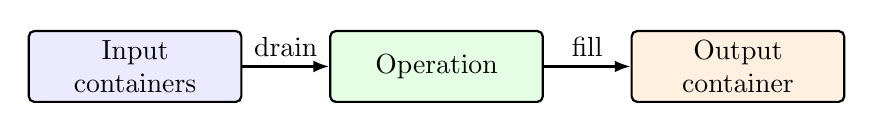
\begin{tikzpicture}[
        box/.style={draw, thick, rounded corners=2pt, minimum width=2.7cm, minimum height=0.9cm, align=center},
        arrow/.style={-{Latex[length=2mm]}, thick}
      ]
      \node[box, fill=blue!8] (in) {Input\\containers};
      \node[box, fill=green!10, right=1.1cm of in] (op) {Operation};
      \node[box, fill=orange!12, right=1.1cm of op] (out) {Output\\container};
      \draw[arrow] (in) -- node[above]{drain} (op);
      \draw[arrow] (op) -- node[above]{fill} (out);
    \end{tikzpicture}
  \end{center}

  \vspace{0.25cm}
  \begin{itemize}
    \item An operation consumes one or more input values from containers.
    \item It produces one output value into another container.
    \item It can start only when its input values are ready and its output container is free.
    \item Once an input has been fully drained, its container is free to reuse.
    \item Once the output has been fully computed, it is ready to be consumed.
  \end{itemize}
\end{frame}

\begin{frame}{When Can an Operation Start?}
  An operation is schedulable only when both conditions are true:

  \vspace{0.25cm}
  \begin{enumerate}
    \item \textbf{Input value-ready}: every input value it needs has been produced.
    \item \textbf{Output resource-free}: the container for its output is available.
  \end{enumerate}

  \vspace{0.3cm}
  In other words, the operation is blocked if either the data is not ready
  or the destination container is still occupied.

  \vspace{0.25cm}
  This is the basic rule behind SMEM ring-buffer reuse, TMEM reuse, and TMA
  store-buffer pipelining.
\end{frame}

\begin{frame}{Two Signals}
  In this model, synchronization has two meanings:

  \begin{enumerate}
    \item \textbf{Value-ready}: a container is full; its value can be consumed.
    \item \textbf{Resource-free}: a container is empty; it can be reused.
  \end{enumerate}

  \vspace{0.3cm}
  A producer is waiting for a free output container. A consumer is waiting for
  a ready input value. Good GEMM scheduling is mostly about making those two
  waits overlap with useful work.

  \vspace{0.15cm}
  For TMEM, value readiness is gated by a named completion signal:
  \textbf{all-MMAs-done}. A single MMA finishing is not enough.

  \vspace{0.25cm}
  \begin{center}
    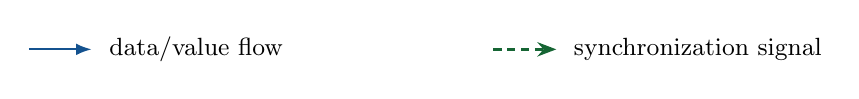
\begin{tikzpicture}[
        flow/.style={-{Latex[length=2mm]}, thick},
        signal/.style={-{Stealth[length=2.4mm]}, very thick, densely dashed}
      ]
      \draw[flow, draw=mmblue] (-4.6,0) -- (-3.8,0);
      \node[right] at (-3.7,0) {\small data/value flow};
      \draw[signal, draw=mmgreen] (1.3,0) -- (2.1,0);
      \node[right] at (2.2,0) {\small synchronization signal};
    \end{tikzpicture}
  \end{center}
\end{frame}

\begin{frame}{Dataflow Alone Is Not Enough}
  The high-level dataflow is simple:

  \vspace{0.3cm}
  \begin{center}
    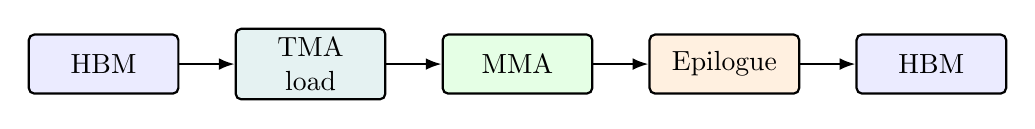
\begin{tikzpicture}[
        node/.style={draw, thick, rounded corners=2pt, minimum width=1.9cm, minimum height=0.75cm, align=center},
        arrow/.style={-{Latex[length=2mm]}, thick}
      ]
      \node[node, fill=blue!8] (hbm0) {HBM};
      \node[node, fill=teal!10, right=0.7cm of hbm0] (tma) {TMA\\load};
      \node[node, fill=green!10, right=0.7cm of tma] (mma) {MMA};
      \node[node, fill=orange!12, right=0.7cm of mma] (epi) {Epilogue};
      \node[node, fill=blue!8, right=0.7cm of epi] (hbm1) {HBM};
      \draw[arrow] (hbm0) -- (tma);
      \draw[arrow] (tma) -- (mma);
      \draw[arrow] (mma) -- (epi);
      \draw[arrow] (epi) -- (hbm1);
    \end{tikzpicture}
  \end{center}

  \vspace{0.3cm}
  But this diagram hides the most important scheduling question:

  \vspace{0.15cm}
  \begin{center}
    \textbf{Where is each value stored while it waits for the next operation?}
  \end{center}
\end{frame}

\begin{frame}{Add the Containers}
  For the framework used in this talk, the main containers are:

  \begin{table}
    \centering
    \small
    \begin{tabular}{lll}
      \toprule
      Operation & Input container & Output container \\
      \midrule
      TMA load & HBM A/B tiles & SMEM compute ring buffer \\
      MMA & SMEM compute ring buffer & TMEM accumulator \\
      Epilogue drain & TMEM accumulator & Registers \\
      Epilogue pack & Registers & SMEM store ring buffer \\
      TMA store & SMEM store ring buffer & HBM C tile \\
      \bottomrule
    \end{tabular}
  \end{table}

  \vspace{0.2cm}
  This is the concrete dataflow graph: operations connected by values, and
  each value stored in an explicit container.
\end{frame}

\begin{frame}[fragile]{Main Synchronization Pattern}
  \small
  \begin{verbatim}
  +------+    +-----------+    +---------------------+
  | HBM  | -> | TMA warps | -> | SMEM compute buffer |
  +------+    +-----------+    +---------------------+
                  |  SMEM full               ^
                  v                           | SMEM free
  +------+    +-----------+    +------+
  | SMEM | -> | MMA warps | -> | TMEM |
  +------+    +-----------+    +------+
                  |  TMEM full*              ^
                  |                           | TMEM free
                  v                           |
  +------+    +----------------+    +-----------+
  | TMEM | -> | epilogue warps | -> | registers |
  +------+    +----------------+    +-----------+
  \end{verbatim}
  \vspace{-0.2cm}
  {* `TMEM full' is sent only after the final MMA finishes.}
\end{frame}

\begin{frame}{Main Synchronization Pattern: Graph View}
  \begin{center}
    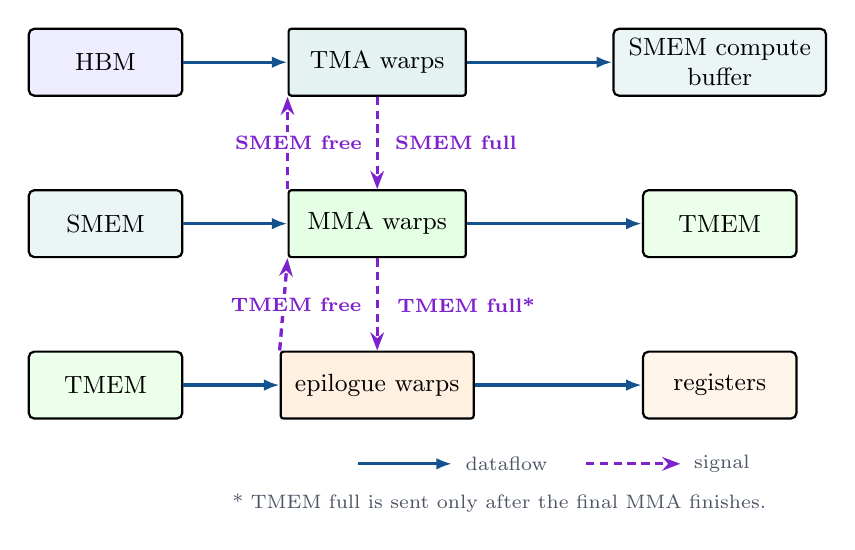
\begin{tikzpicture}[
        container/.style={draw, thick, rounded corners=2pt, minimum width=1.95cm, minimum height=0.85cm, align=center, font=\small},
        op/.style={draw, thick, rounded corners=1pt, minimum width=2.25cm, minimum height=0.85cm, align=center, font=\small},
        flow/.style={-{Latex[length=2mm]}, very thick, draw=mmblue},
        signal/.style={-{Stealth[length=2.3mm]}, very thick, densely dashed},
        siglabel/.style={font=\scriptsize\bfseries, inner sep=1.5pt, fill=white}
      ]
      \node[container, fill=blue!7] (hbm1) at (-5.0,2.05) {HBM};
      \node[op, fill=teal!10] (tma) at (-1.55,2.05) {TMA warps};
      \node[container, fill=teal!8, minimum width=2.7cm] (smem1) at (2.8,2.05) {SMEM compute\\buffer};

      \node[container, fill=teal!8] (smem2) at (-5.0,0) {SMEM};
      \node[op, fill=green!10] (mma) at (-1.55,0) {MMA warps};
      \node[container, fill=green!8] (tmem2) at (2.8,0) {TMEM};

      \node[container, fill=green!8] (tmem3) at (-5.0,-2.05) {TMEM};
      \node[op, fill=orange!12, minimum width=2.45cm] (epi) at (-1.55,-2.05) {epilogue warps};
      \node[container, fill=orange!8] (regs) at (2.8,-2.05) {registers};

      \draw[flow] (hbm1) -- (tma);
      \draw[flow] (tma) -- (smem1);
      \draw[flow] (smem2) -- (mma);
      \draw[flow] (mma) -- (tmem2);
      \draw[flow] (tmem3) -- (epi);
      \draw[flow] (epi) -- (regs);

      \draw[signal, draw=mmsignal] (tma.south) -- (mma.north);
      \node[siglabel, text=mmsignal] at (-0.55,1.03) {SMEM full};

      \draw[signal, draw=mmsignal] (mma.north west) -- (tma.south west);
      \node[siglabel, text=mmsignal] at (-2.55,1.03) {SMEM free};

      \draw[signal, draw=mmsignal] (mma.south) -- (epi.north);
      \node[siglabel, text=mmsignal] at (-0.42,-1.03) {TMEM full*};

      \draw[signal, draw=mmsignal] (epi.north west) -- (mma.south west);
      \node[siglabel, text=mmsignal] at (-2.58,-1.03) {TMEM free};

      \draw[flow] (-1.8,-3.05) -- (-0.6,-3.05);
      \node[font=\scriptsize, text=mmgray, right] at (-0.55,-3.05) {dataflow};
      \draw[signal, draw=mmsignal] (1.1,-3.05) -- (2.3,-3.05);
      \node[font=\scriptsize, text=mmgray, right] at (2.35,-3.05) {signal};
      \node[font=\scriptsize, text=mmgray, align=center] at (0,-3.55)
        {* TMEM full is sent only after the final MMA finishes.};
    \end{tikzpicture}
  \end{center}
\end{frame}

\begin{frame}{TMA Warp: Drain HBM, Fill SMEM}
  \begin{center}
    \begin{tikzpicture}[
        container/.style={circle, draw, thick, minimum size=2.25cm, align=center},
        op/.style={draw, thick, rounded corners=1pt, minimum width=1.65cm, minimum height=1.2cm, align=center},
        arrow/.style={-{Latex[length=2mm]}, very thick},
        status/.style={font=\scriptsize, text=mmgray},
        fillhbm/.style={fill=blue!25, draw=none},
        fillsmem/.style={fill=teal!35, draw=none}
      ]
      \node[container, fill=blue!6] (hbm) at (-4.4,0) {};
      \node[op, fill=teal!10] (tma) at (0,0) {TMA\\warp};
      \node[container, fill=teal!7] (smem) at (4.4,0) {};

      \draw[arrow, draw=mmblue] (hbm) -- node[above]{drain} (tma);
      \draw[arrow, draw=mmblue] (tma) -- node[above]{fill} (smem);

      \begin{scope}
        \clip (-4.4,0) circle (1.125cm);
        \only<1>{\fill[fillhbm] (-5.525,-1.125) rectangle (-3.275,1.125);}
        \only<2>{\fill[fillhbm] (-5.525,-1.125) rectangle (-3.275,0);}
      \end{scope}

      \begin{scope}
        \clip (4.4,0) circle (1.125cm);
        \only<2>{\fill[fillsmem] (3.275,-1.125) rectangle (5.525,0);}
        \only<3>{\fill[fillsmem] (3.275,-1.125) rectangle (5.525,1.125);}
      \end{scope}

      \node[align=center] at (hbm) {HBM\\tile};
      \node[align=center] at (smem) {SMEM\\compute\\buffer};

      \node[status, below=0.1cm of hbm] {
        \only<1>{full}
        \only<2>{half drained}
        \only<3>{empty}
      };
      \node[status, below=0.1cm of smem] {
        \only<1>{empty}
        \only<2>{half full}
        \only<3>{full}
      };

      \node[align=center, text width=11cm] at (0,-2.1) {
        \only<1>{The TMA warp can start: the HBM tile is ready and the SMEM output container is free.}
        \only<2>{The input container is being drained while the output container is being filled.}
        \only<3>{The HBM input is drained, and the SMEM compute buffer now contains the produced tile.}
      };
    \end{tikzpicture}
  \end{center}
\end{frame}

\begin{frame}{TMA Warp: Output Signal}
  \begin{center}
    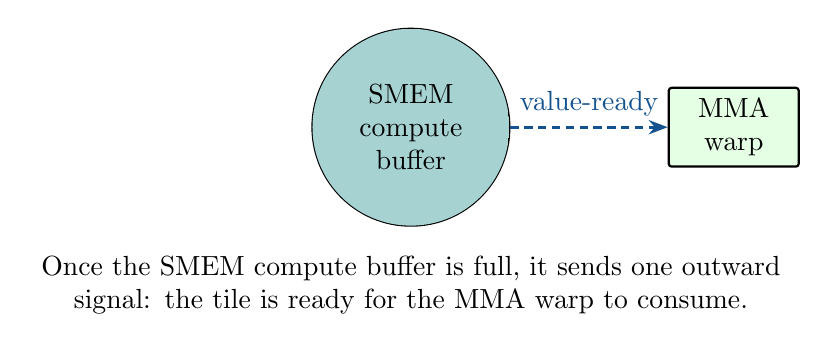
\begin{tikzpicture}[
        container/.style={circle, draw, thick, minimum size=2.5cm, align=center},
        op/.style={draw, thick, rounded corners=1pt, minimum width=1.65cm, minimum height=1.0cm, align=center},
        signal/.style={-{Stealth[length=2.4mm]}, very thick, densely dashed},
        fillsmem/.style={fill=teal!35, draw=none}
      ]
      \node[container, fill=teal!7] (smem) at (0,0) {};
      \begin{scope}
        \clip (0,0) circle (1.25cm);
        \fill[fillsmem] (-1.25,-1.25) rectangle (1.25,1.25);
      \end{scope}
      \node[align=center] at (smem) {SMEM\\compute\\buffer};
      \node[op, fill=green!10] (mma) at (4.1,0) {MMA\\warp};
      \draw[signal, draw=mmblue, text=mmblue] (smem) -- node[above]{value-ready} (mma);

      \node[align=center, text width=9.5cm] at (0,-2.0) {
        Once the SMEM compute buffer is full, it sends one outward signal:
        the tile is ready for the MMA warp to consume.
      };
    \end{tikzpicture}
  \end{center}
\end{frame}

\begin{frame}{MMA Warp: Drain SMEM, Fill TMEM}
  \begin{center}
    \begin{tikzpicture}[
        container/.style={circle, draw, thick, minimum size=2.25cm, align=center},
        op/.style={draw, thick, rounded corners=1pt, minimum width=1.65cm, minimum height=1.2cm, align=center},
        arrow/.style={-{Latex[length=2mm]}, very thick},
        status/.style={font=\scriptsize, text=mmgray},
        fillsmem/.style={fill=teal!35, draw=none},
        filltmem/.style={fill=green!35, draw=none}
      ]
      \node[container, fill=teal!7] (smem) at (-4.4,0) {};
      \node[op, fill=green!10] (mma) at (0,0) {MMA\\warp};
      \node[container, fill=green!7] (tmem) at (4.4,0) {};

      \draw[arrow, draw=mmblue] (smem) -- node[above]{drain} (mma);
      \draw[arrow, draw=mmblue] (mma) -- node[above]{fill} (tmem);

      \begin{scope}
        \clip (-4.4,0) circle (1.125cm);
        \only<1>{\fill[fillsmem] (-5.525,-1.125) rectangle (-3.275,1.125);}
        \only<2>{\fill[fillsmem] (-5.525,-1.125) rectangle (-3.275,0);}
      \end{scope}

      \begin{scope}
        \clip (4.4,0) circle (1.125cm);
        \only<2>{\fill[filltmem] (3.275,-1.125) rectangle (5.525,0);}
        \only<3>{\fill[filltmem] (3.275,-1.125) rectangle (5.525,1.125);}
      \end{scope}

      \node[align=center] at (smem) {SMEM\\compute\\buffer};
      \node[align=center] at (tmem) {TMEM\\buffer};

      \node[status, below=0.1cm of smem] {
        \only<1>{full}
        \only<2>{half drained}
        \only<3>{empty}
      };
      \node[status, below=0.1cm of tmem] {
        \only<1>{empty}
        \only<2>{half full}
        \only<3>{full}
      };

      \node[align=center, text width=11cm] at (0,-2.1) {
        \only<1>{The MMA warp can start: the SMEM tile is ready and the TMEM output container is free.}
        \only<2>{MMA drains the SMEM compute buffer while filling the TMEM accumulator.}
        \only<3>{The SMEM input is empty, and the TMEM output is full.}
      };
    \end{tikzpicture}
  \end{center}
\end{frame}

\begin{frame}{MMA Warp: Output and Reuse Signals}
  \begin{center}
    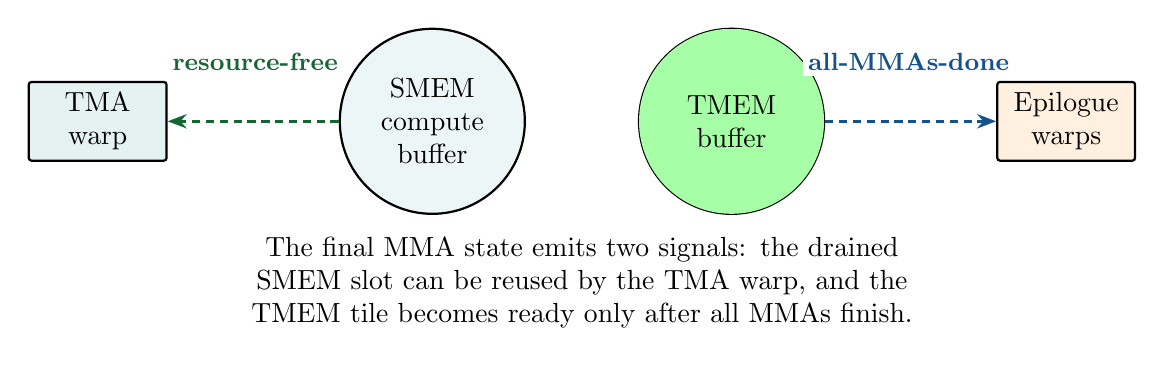
\begin{tikzpicture}[
        container/.style={circle, draw, thick, minimum size=2.35cm, align=center},
        op/.style={draw, thick, rounded corners=1pt, minimum width=1.75cm, minimum height=1.0cm, align=center},
        siglabel/.style={font=\small\bfseries, inner sep=2pt, fill=white},
        signal/.style={-{Stealth[length=2.4mm]}, very thick, densely dashed},
        fillsmem/.style={fill=teal!35, draw=none},
        filltmem/.style={fill=green!35, draw=none}
      ]
      \node[container, fill=teal!7] (smem) at (-1.9,0) {SMEM\\compute\\buffer};
      \node[container, fill=green!7] (tmem) at (1.9,0) {};
      \begin{scope}
        \clip (1.9,0) circle (1.175cm);
        \fill[filltmem] (0.725,-1.175) rectangle (3.075,1.175);
      \end{scope}
      \node[align=center] at (tmem) {TMEM\\buffer};

      \node[op, fill=teal!10] (tma) at (-6.15,0) {TMA\\warp};
      \node[op, fill=orange!12] (epi) at (6.15,0) {Epilogue\\warps};
      \draw[signal, draw=mmgreen] (smem) -- (tma);
      \draw[signal, draw=mmblue] (tmem) -- (epi);
      \node[siglabel, text=mmgreen] at (-4.15,0.75) {resource-free};
      \node[siglabel, text=mmblue] at (4.15,0.75) {all-MMAs-done};

      \node[align=center, text width=10.5cm] at (0,-2.05) {
        The final MMA state emits two signals: the drained SMEM slot can be reused
        by the TMA warp, and the TMEM tile becomes ready only after all MMAs finish.
      };
    \end{tikzpicture}
  \end{center}
\end{frame}

\begin{frame}{Epilogue Warps: Drain TMEM, Fill Registers}
  \begin{center}
    \begin{tikzpicture}[
        container/.style={circle, draw, thick, minimum size=2.25cm, align=center},
        op/.style={draw, thick, rounded corners=1pt, minimum width=1.85cm, minimum height=1.2cm, align=center},
        arrow/.style={-{Latex[length=2mm]}, very thick},
        signal/.style={-{Stealth[length=2.4mm]}, very thick, densely dashed},
        siglabel/.style={font=\small\bfseries, inner sep=2pt, fill=white},
        status/.style={font=\scriptsize, text=mmgray},
        filltmem/.style={fill=green!35, draw=none},
        fillregs/.style={fill=orange!35, draw=none}
      ]
      \node[container, fill=green!7] (tmem) at (-4.4,0) {};
      \node[op, fill=orange!12] (epi) at (0,0) {Epilogue\\warps};
      \node[container, fill=orange!8] (regs) at (4.4,0) {};

      \draw[arrow, draw=mmblue] (tmem) -- node[above]{drain} (epi);
      \draw[arrow, draw=mmblue] (epi) -- node[above]{fill} (regs);

      \begin{scope}
        \clip (-4.4,0) circle (1.125cm);
        \only<1>{\fill[filltmem] (-5.525,-1.125) rectangle (-3.275,1.125);}
        \only<2>{\fill[filltmem] (-5.525,-1.125) rectangle (-3.275,0);}
      \end{scope}

      \begin{scope}
        \clip (4.4,0) circle (1.125cm);
        \only<2>{\fill[fillregs] (3.275,-1.125) rectangle (5.525,0);}
        \only<3>{\fill[fillregs] (3.275,-1.125) rectangle (5.525,1.125);}
      \end{scope}

      \node[align=center] at (tmem) {TMEM\\buffer};
      \node[align=center] at (regs) {Register\\buffer};

      \node[status, below=0.1cm of tmem] {
        \only<1>{full}
        \only<2>{half drained}
        \only<3>{empty}
      };
      \node[status, below=0.1cm of regs] {
        \only<1>{empty}
        \only<2>{half full}
        \only<3>{full}
      };

      \node[op, fill=green!10] (mma) at (0,1.75) {MMA\\warps};
      \only<1>{
        \draw[signal, draw=mmblue] (mma) -- (epi);
        \node[siglabel, text=mmblue] at (2.15,1.0) {all-MMAs-done};
      }

      \node[align=center, text width=11cm] at (0,-2.1) {
        \only<1>{The epilogue can start only after all MMAs are done and the register output container is free.}
        \only<2>{The epilogue drains the final TMEM tile while filling registers.}
        \only<3>{After the drain, TMEM is empty and the values are now in registers.}
      };
    \end{tikzpicture}
  \end{center}
\end{frame}

\begin{frame}{Epilogue Warps: TMEM Reuse Signal}
  \begin{center}
    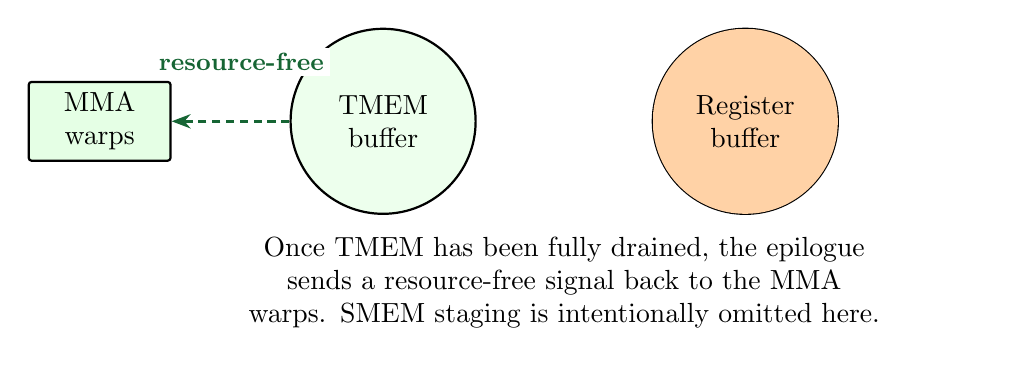
\begin{tikzpicture}[
        container/.style={circle, draw, thick, minimum size=2.35cm, align=center},
        op/.style={draw, thick, rounded corners=1pt, minimum width=1.8cm, minimum height=1.0cm, align=center},
        signal/.style={-{Stealth[length=2.4mm]}, very thick, densely dashed},
        siglabel/.style={font=\small\bfseries, inner sep=2pt, fill=white},
        fillregs/.style={fill=orange!35, draw=none}
      ]
      \node[container, fill=green!7] (tmem) at (-2.3,0) {TMEM\\buffer};
      \node[container, fill=orange!8] (regs) at (2.3,0) {};
      \begin{scope}
        \clip (2.3,0) circle (1.175cm);
        \fill[fillregs] (1.125,-1.175) rectangle (3.475,1.175);
      \end{scope}
      \node[align=center] at (regs) {Register\\buffer};

      \node[op, fill=green!10] (mma) at (-5.9,0) {MMA\\warps};
      \draw[signal, draw=mmgreen] (tmem) -- (mma);
      \node[siglabel, text=mmgreen] at (-4.1,0.75) {resource-free};

      \node[align=center, text width=10.5cm] at (0,-2.05) {
        Once TMEM has been fully drained, the epilogue sends a resource-free
        signal back to the MMA warps. SMEM staging is intentionally omitted here.
      };
    \end{tikzpicture}
  \end{center}
\end{frame}

\begin{frame}{Deriving the Warp Roles}
  \begin{table}
    \centering
    \small
    \begin{tabular}{llll}
      \toprule
      Worker & Drains & Fills & Key signal \\
      \midrule
      TMA warp & HBM tile & SMEM compute ring & tile ready \\
      MMA warp & SMEM compute ring & TMEM & SMEM free / all-MMAs-done \\
      Epilogue warp & TMEM & registers & TMEM free \\
      TMA store path & SMEM store ring & HBM output & store slot free \\
      \bottomrule
    \end{tabular}
  \end{table}

  \vspace{0.2cm}
  The same rule repeats: drain an input container, fill an output container,
  then signal readiness, completion, or resource reuse.
\end{frame}

\section{2-CTA MMA}

\begin{frame}{One Optimization the Model Does Not Imply: 2-CTA MMA}
  The orchestration model already covers warp specialization, pipelining,
  SMEM/TMEM reuse, and epilogue overlap. One major B200 optimization is
  \emph{not} implied by it:

  \vspace{0.3cm}
  \begin{center}
    \textbf{2-CTA MMA}: two CTAs in a cluster cooperate on one MMA.
  \end{center}

  \vspace{0.3cm}
  \begin{itemize}
    \item Form a cluster of 2 CTAs (\code{\_\_cluster\_dims\_\_(2,1,1)}).
    \item Issue a single \code{tcgen05.mma.cta\_group::2} across the pair.
    \item The pair produces a $2\,BM \times BN$ output tile per MMA.
  \end{itemize}
\end{frame}

\begin{frame}{2-CTA MMA: Geometry}
  \begin{columns}[T,onlytextwidth]
    \column{0.52\textwidth}
    \begin{itemize}
      \item Each CTA owns \textbf{half of B}: $BN_{\text{local}} = BN/2$.
      \item Both CTAs load the \textbf{full A} rows for their $BM$.
      \item Per-CTA SMEM per slot drops from 48\,KB to \textbf{32\,KB} (at $BN{=}256$).
      \item TMA loads use \code{.cta\_group::2}; the \code{tcgen05.commit}
        multicasts the completion signal to both CTAs.
    \end{itemize}

    \column{0.46\textwidth}
    \begin{center}
      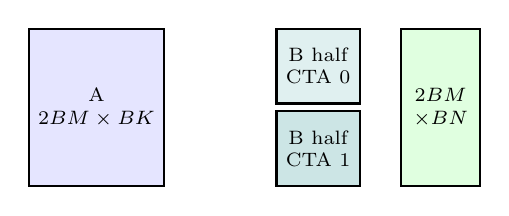
\begin{tikzpicture}[box/.style={draw, thick, align=center, font=\scriptsize}]
        \node[box, fill=blue!10, minimum width=1.4cm, minimum height=2.0cm] (a) {A\\$2BM\times BK$};
        \node[box, fill=teal!12, minimum width=1.0cm, minimum height=0.95cm, right=1.4cm of a.north east, anchor=north west] (b0) {B half\\CTA 0};
        \node[box, fill=teal!20, minimum width=1.0cm, minimum height=0.95cm, below=2pt of b0] (b1) {B half\\CTA 1};
        \node[box, fill=green!12, minimum width=1.0cm, minimum height=2.0cm, right=0.5cm of b0.north east, anchor=north west] (c) {$2BM$\\$\times BN$};
      \end{tikzpicture}
    \end{center}
  \end{columns}
\end{frame}

\begin{frame}[fragile]{2-CTA MMA: In the Instructions}
  The cluster cooperation shows up directly in the PTX:
  \begin{lstlisting}[language=C]
// TMA load into clustered SMEM (both CTAs' arrivals counted):
cp.async.bulk.tensor.2d.shared::cluster.global
    .mbarrier::complete_tx::bytes.cta_group::2  [smem], [tmap,{x,y}], [mbar];

// One MMA issued across the CTA pair:
tcgen05.mma.cta_group::2.kind::f16  ... ;

// Completion multicast to both CTAs in the cluster:
tcgen05.commit.cta_group::2.mbarrier::arrive::one
    .shared::cluster.multicast::cluster.b64  [smem_compute_free_mbar], cta_mask;
  \end{lstlisting}
  \vspace{-0.2cm}
  \footnotesize Source: \code{webui/kernels/tier3\_cluster\_swizzle/kernel.cu}.
\end{frame}

\section{Tile Sizes and Shared Memory}

\begin{frame}{Framework Choice: Disjoint SMEM}
  There are several valid ways to share on-chip storage between compute and
  epilogue. In this talk, we will use one common framework:

  \begin{itemize}
    \item Compute uses a dedicated SMEM ring buffer for A/B tiles.
    \item The epilogue is \textbf{always a pipelined TMA store}: it packs results
      into a separate SMEM store ring buffer and lets TMA push tiles to HBM.
    \item The number of TMA store pipeline stages is a tunable parameter.
  \end{itemize}

  \vspace{0.2cm}
  This is not the only possible design, but it is a clean default that works
  well across many shapes. Its consequence: shared memory splits into
  \textbf{two} rings, and 2-CTA tile sizes set how big each one is.
\end{frame}

\begin{frame}{Partitioning Shared Memory}
  \begin{center}
    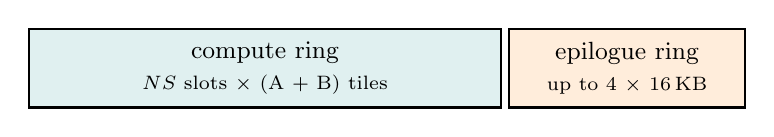
\begin{tikzpicture}[
        seg/.style={draw, thick, minimum height=1.0cm, align=center, font=\small}
      ]
      \node[seg, fill=teal!12, minimum width=6.0cm] (comp) at (0,0)
        {compute ring\\ \scriptsize $NS$ slots $\times$ (A + B) tiles};
      \node[seg, fill=orange!14, minimum width=3.0cm, right=2pt of comp] (epi)
        {epilogue ring\\ \scriptsize up to 4 $\times$ 16\,KB};
    \end{tikzpicture}
  \end{center}

  \vspace{0.1cm}
  \begin{itemize}
    \item \textbf{Compute ring}: $NS$ pipeline slots, each holding one A tile and
      one B tile for the MMA stage.
    \item \textbf{Epilogue ring}: the TMA store buffers. MMComposer exposes up to
      \textbf{4} store buffers, each \textbf{16\,KB}.
    \item Both rings share one per-SM SMEM budget, so larger tiles or deeper
      pipelines on one side leave less room for the other.
  \end{itemize}
\end{frame}

\begin{frame}{Tile Sizes and the SMEM Budget}
  Per compute slot (2-CTA, each CTA owns half of B):
  \[
    \text{slot} = \underbrace{BM\cdot BK\cdot 2}_{\text{A tile}}
                + \underbrace{\tfrac{BN}{2}\cdot BK\cdot 2}_{\text{B tile (local)}}
  \]

  \begin{table}
    \centering\small
    \begin{tabular}{lrrr}
      \toprule
      Config (2-CTA, $BK{=}64$) & A tile & B tile & slot \\
      \midrule
      $BM{=}128,\ BN{=}256$ & 16\,KB & 16\,KB & 32\,KB \\
      $BM{=}128,\ BN{=}512$ & 16\,KB & 32\,KB & 48\,KB \\
      \bottomrule
    \end{tabular}
  \end{table}

  \vspace{0.15cm}
  Budget constraint (per SM, B200 $\approx$ 228\,KB):
  \[
    \underbrace{NS \times \text{slot}}_{\text{compute ring}}
    \;+\;
    \underbrace{E \times 16\,\text{KB}}_{\text{epilogue ring},\ E\le 4}
    \;\le\; S_{\text{SMEM}}
  \]

  \footnotesize Example: $BN{=}256$, $NS{=}5 \Rightarrow 160$\,KB compute ring;
  with $E{=}2$ store buffers, $+32$\,KB $= 192$\,KB total.
  % TODO(tong): confirm the exact per-SM SMEM cap used (228 KB?).
\end{frame}

\section{From Diagram to Code}

\begin{frame}{From Diagram to Code}
  We now connect the container diagram to the real kernel. Each warp role maps
  to one loop that \emph{waits}, \emph{works}, then \emph{signals}:

  \vspace{0.3cm}
  \begin{table}
    \centering\scriptsize
    \begin{tabular}{llll}
      \toprule
      Warp & Waits on & Works & Signals \\
      \midrule
      TMA & \code{smem\_compute\_free\_mbar[slot]} & TMA load A/B & \code{smem\_compute\_full\_mbar[slot]} \\
      MMA & \code{smem\_compute\_full\_mbar[slot]} & \code{tcgen05.mma} & \code{smem\_compute\_free\_mbar}, \code{tmem\_full} \\
      Epilogue & \code{tmem\_full[buf]} & drain + TMA store & \code{tmem\_free\_mbar[buf]} \\
      \bottomrule
    \end{tabular}
  \end{table}

  \vspace{0.2cm}
  The mbarriers \emph{are} the dashed signal arrows from the diagrams.
\end{frame}

\begin{frame}[fragile]{TMA Warp: Fill SMEM, Signal Ready}
  \begin{lstlisting}[language=C]
if (warp_id == 0 && elect_sync()) {            // TMA-load warp
  for (int k = 0; k < num_k; k++) {
    int slot = gk % NS;
    mbarrier_wait_phase(smem_compute_free_mbar[slot],
                        smem_compute_free_phase[slot]); // wait: SMEM free
    tma_2d_load_g2(A_base(slot), A_tmap, ...);        // drain HBM -> fill A
    tma_2d_load_g2(B_base(slot), B_tmap, ...);        //              fill B
    mbarrier_arrive_expect_tx(smem_compute_full_mbar[slot],
                              SLOT_BYTES);            // signal: SMEM full
    gk++;
  }
}
  \end{lstlisting}
  \vspace{-0.2cm}
  \footnotesize Wait on \emph{resource-free}, fill, then send \emph{value-ready}.
\end{frame}

\begin{frame}[fragile]{MMA Warp: Consume SMEM, Signal All-MMAs-Done}
  \begin{lstlisting}[language=C]
else if (cta_rank == 0 && warp_id == 1 && elect_sync()) {   // MMA warp
  mbarrier_wait_phase(tmem_free_mbar[buf],
                      tmem_free_phase[buf]);        // wait: TMEM free
  for (int k = 0; k < num_k; k++) {
    int slot = gk % NS;
    mbarrier_wait_phase(smem_compute_full_mbar[slot],
                        smem_compute_full_phase[slot]); // wait: SMEM full
    issue_mma_chain(d_tmem, A_base(slot), B_base(slot), ...);
    tcgen05_commit_mcast_g2(smem_compute_free_mbar[slot],
                            cta_mask);              // signal: SMEM free
    gk++;
  }
  tcgen05_commit_mcast_g2(tmem_full[buf], cta_mask);   // signal: all-MMAs-done
}
  \end{lstlisting}
\end{frame}

\begin{frame}[fragile]{Epilogue Warps: Drain TMEM, Pipelined Store}
  \begin{lstlisting}[language=C]
else if (warp_id >= 4 && warp_id < NUM_WARPS + 4) {   // epilogue warps
  mbarrier_wait_phase(tmem_full[buf], full[buf]);  // wait: all-MMAs-done
  tcgen05_ld(...);                                 // drain TMEM -> registers
  // pack registers -> SMEM store ring -> cp.async.bulk.tensor.2d (TMA store)
  EPI_TMEM_FREE_ARRIVE();                           // signal: TMEM free
}
  \end{lstlisting}
  \vspace{-0.2cm}
  \footnotesize The store ring is the epilogue half of the SMEM partition; TMA
  drains it to HBM asynchronously.
\end{frame}

\section{MMComposer}

\begin{frame}{What MMComposer Generates}
  MMComposer is a code generator: from a knob configuration it emits a
  specialized \code{kernel.cu} (and a self-contained host driver).

  \begin{itemize}
    \item Skeletons are organized as \textbf{tiers}:
      \begin{itemize}
        \item Tier 1 --- baseline (no warp specialization).
        \item Tier 2 --- multi-stage + warp specialization (single CTA).
        \item Tier 3 --- + 2-CTA cluster MMA.
      \end{itemize}
    \item Each knob (tile size, stages, epilogue mode, \ldots) is substituted
      into the skeleton at generation time.
    \item The generated kernel is exactly the orchestration pipeline from the
      earlier diagrams.
  \end{itemize}
\end{frame}

\begin{frame}{Using MMComposer: WebUI Knobs}
  \begin{columns}[T,onlytextwidth]
    \column{0.5\textwidth}
    \textbf{Geometry}
    \begin{itemize}
      \item \code{BM} (128), \code{BN} (64--512), \code{BK} (64)
      \item \code{NS}: pipeline depth (2--7)
      \item \code{NUM\_WARPS} (4/8/16), \code{GROUP\_SIZE\_M}
    \end{itemize}
    \textbf{Structure}
    \begin{itemize}
      \item Multi-stage + warp specialization
      \item 2-CTA cluster MMA
      \item Persistent grid
    \end{itemize}
    \column{0.5\textwidth}
    \textbf{Epilogue}
    \begin{itemize}
      \item Epilogue overlap (TMEM double-buffer)
      \item Pipelined TMA-store epilogue
      \item \code{TMA\_STORE\_STAGES} (1--4)
      \item Split writeback, L1 no-allocate
      \item Single-TMEM accumulator
    \end{itemize}
  \end{columns}

  \vspace{0.2cm}
  \footnotesize Run with \code{streamlit run webui/app.py}.
\end{frame}

\begin{frame}[fragile]{Using MMComposer: CLI}
  Generate a kernel or host driver from a config JSON:
  \begin{lstlisting}[language=bash]
python -m codegen kernel config.json   > kernel.cu
python -m codegen host   config.json   > host.py
  \end{lstlisting}
  \begin{lstlisting}
{
  "skeleton": "tier3_cluster_swizzle",
  "BM": 128, "BN": 256, "BK": 64,
  "NS": 5, "GROUP_SIZE_M": 4, "NUM_WARPS": 8,
  "EPILOGUE_OVERLAP": 1, "EPILOGUE_TMA_PIPELINED": 1,
  "TMA_STORE_STAGES": 2, "TWO_CTA": 1
}
  \end{lstlisting}
\end{frame}

\begin{frame}[fragile]{Autotuning}
  Sweep the knob grid on a B200 and rank by TFLOPS vs cuBLAS:
  \begin{lstlisting}[language=bash]
python webui/autotune.py 8192                    # square 8192^3
python webui/autotune.py 32768x4608x768          # MxNxK
python webui/autotune.py 8192 --scope production # filtered grid
  \end{lstlisting}
  \begin{lstlisting}
cuBLAS reference: 1567 TFLOPS
  #  TFLOPS  %cuBLAS   WS 2CTA  BN  NS GSM  NW  TMS
---- ------- ------- --- ----  --- -- --- --  ---
  1  1456.0  92.9%   on   on  256  5   4   4   2
  2  1398.0  89.2%   on   on  256  4   4   4   2
  3  1345.0  85.8%   on   on  512  4   8   8   2
  \end{lstlisting}
  \vspace{-0.2cm}
  \footnotesize \emph{production} scope filters to warp-spec, \code{BN}$\in\{256,512\}$,
  \code{NS}$\ge 3$.
\end{frame}


\end{document}
